%%%%%%%%%%%%%%%%%%%%%%%%%%%%%%%%%%%%%%%%%%%%%%%%%%%%%%%%
%%%%%%%%%%%%%%%%%%%%%%%%%%%%%%%%%%%%%%%%%%%%%%%%%%%%%%%%
%%%%%%%%%%%%%%%%%%%%%%%%%%%%%%%%%%%%%%%%%%%%%%%%%%%%%%%%
%%%%%%%%%%%%%%%%%%%%%%%%%%%%%%%%%%%%%%%%%%%%%%%%%%%%%%%%
\documentclass[a4paper,12pt,twoside,openright]{report}
\usepackage[bibjustif]{abntex2cite}
\usepackage[brazil]{babel}
\usepackage{setspace}
\usepackage{amsthm}
\usepackage{mathtools}
\usepackage[figuresright]{rotating}
\usepackage{graphics}
\usepackage{amssymb}
\usepackage{graphicx}
\usepackage{fancybox}
\usepackage{amsmath}
\usepackage{picinpar}
\usepackage{colortbl}
\usepackage{wasysym}
\usepackage{txfonts}
\usepackage{pb-diagram}
\usepackage{relsize}
\usepackage{tikz}
\usepackage{pgfplots}
\usepackage{subfigure}
\usepackage{algorithm}
\usepackage{algorithmic}
\DeclarePairedDelimiter\ceil{\lceil}{\rceil}
\DeclarePairedDelimiter\floor{\lfloor}{\rfloor}
\usepackage[hang,small,bf]{caption}
\usepackage[compact]{titlesec}
\usepackage[left=3cm,top=3cm,right=2cm,bottom=3cm]{geometry}%esq e sup 3cm  ; dir e inf 2cm
\usepackage[subfigure]{tocloft}
\usepackage{subfigure}
\renewcommand{\cftfigfont}{Figura }
\renewcommand{\cfttabfont}{Tabela }
\renewcommand{\cftfigaftersnum}{ - }
\renewcommand{\cfttabaftersnum}{ - }
\captionsetup{font=footnotesize,labelsep=endash}
\def\baselinestretch{1.6}
\pagestyle{myheadings}
\usepackage{enumitem}
\setlist[enumerate]{label*=\arabic*.}
\begin{document}
\titlespacing{\section}{0cm}{1.5cm}{1.5cm}
\titlespacing{\subsection}{0cm}{1.5cm}{1.5cm}
%%%%%%%%%%%%%%%%%%%%%%%%%%%%%%%%%%%%%%%%%%%%%%%%%%%%%%%%
%%%%%%%%%%%%%%%%%%%%%%%%%%%%%%%%%%%%%%%%%%%%%%%%%%%%%%%%
% CAPA
%%%%%%%%%%%%%%%%%%%%%%%%%%%%%%%%%%%%%%%%%%%%%%%%%%%%%%%%
%%%%%%%%%%%%%%%%%%%%%%%%%%%%%%%%%%%%%%%%%%%%%%%%%%%%%%%%
\setboolean{@twoside}{true}
\title{
	\vspace*{-120pt}
	\hspace*{+55pt}Universidade Estadual Paulista
	\newline
	\hspace*{+45pt}Instituto de Bioci\^{e}ncias, Letras e Ci\^{e}ncias Exatas
	\newline
	\hspace*{+50pt}Departamento de Ci\^{e}ncia da Computa\c{c}\~{a}o e Estat\'{i}stica
	\newline
	\newline
	\newline
	\hspace*{+50pt}Luis Fernando Teixeira Silva
	\newline
	\newline
	\newline
	Um sistema para reconhecimento de comandos falados dependente do locutor
}
\author{{\tiny .}}
\date{\vspace*{+60pt}S\~{a}o Jos\'{e} do Rio Preto - SP \\ 2017}
\maketitle
\newpage
\thispagestyle{empty}
%%%%%%%%%%%%%%%%%%%%%%%%%%%%%%%%%%%%%%%%%%%%%%%%%%%%%%%%
%%%%%%%%%%%%%%%%%%%%%%%%%%%%%%%%%%%%%%%%%%%%%%%%%%%%%%%%
% PAGINA DE ROSTO
%%%%%%%%%%%%%%%%%%%%%%%%%%%%%%%%%%%%%%%%%%%%%%%%%%%%%%%%
%%%%%%%%%%%%%%%%%%%%%%%%%%%%%%%%%%%%%%%%%%%%%%%%%%%%%%%%
\pagestyle{empty}
\begin{tabular}{p{430pt}}
\pagestyle{empty}
\begin{center}
\pagestyle{empty}
\LARGE{\hspace*{+50pt}Luis Fernando Teixeira Silva\newline \newline \newline \newline \newline Um sistema para reconhecimento de comandos falados dependente do locutor}
\end{center}
\vspace*{+30pt}
\hspace*{+200pt}
\begin{tabular}{p{200pt}}
	\singlespacing{\small Monografia apresentada ao Programa de gradua\c{c}\~{a}o em Ci\^{e}ncia da Computa\c{c}\~{a}o da UNESP para obten\c{c}\~{a}o do t\'{i}tulo de Bacharel. \newline \newline Orientador: Prof. Dr. Rodrigo Capobianco Guido} \\
\end{tabular}
\newline 
\newline
\begin{center}
{\large S\~{a}o Jos\'{e} do Rio Preto - SP \\ 2017}
\end{center}
\end{tabular}
%%%%%%%%%%%%%%%%%%%%%%%%%%%%%%%%%%%%%%%%%%%%%%%%%%%%%%%%
%%%%%%%%%%%%%%%%%%%%%%%%%%%%%%%%%%%%%%%%%%%%%%%%%%%%%%%%
% DEDICATORIA
%%%%%%%%%%%%%%%%%%%%%%%%%%%%%%%%%%%%%%%%%%%%%%%%%%%%%%%%
%%%%%%%%%%%%%%%%%%%%%%%%%%%%%%%%%%%%%%%%%%%%%%%%%%%%%%%%
\newpage
\thispagestyle{empty}
\vspace*{+480pt}
\hspace*{+160pt}
\begin{tabular}{p{200pt}}
	{\small Dedico este trabaho a todos os meus familiares, em especial aos meus pais, Nilda, Luis Carlos e a minha irm\~{a} Ana Beatriz.\newline Dedico tamb\'{e}m esse trabalho para a minha namorada Cristiana Luiza.}
\end{tabular}
%%%%%%%%%%%%%%%%%%%%%%%%%%%%%%%%%%%%%%%%%%%%%%%%%%%%%%%%
%%%%%%%%%%%%%%%%%%%%%%%%%%%%%%%%%%%%%%%%%%%%%%%%%%%%%%%%
% AGRADECIMENTOS
%%%%%%%%%%%%%%%%%%%%%%%%%%%%%%%%%%%%%%%%%%%%%%%%%%%%%%%%
%%%%%%%%%%%%%%%%%%%%%%%%%%%%%%%%%%%%%%%%%%%%%%%%%%%%%%%%
\newpage
\thispagestyle{empty}
\begin{center}{\LARGE \textbf{Agradecimentos}}\end{center}
\vspace{+60pt}
\par Primeiramente, gostaria de agradecer aos meus pais e \`{a} minha madrinha, pois sem o apoio deles eu nunca teria conseguido ter acesso a um ensino de qualidade como aquele que o Cursinho Alternativo me proporcionou durante todo o ano de 2012. Foi gra{\c c}as a essas tr\^{e}s pessoas que pude ingressar nesta linda universidade.
\\
\par Gostaria de agradecer tamb\'{e}m \`{a} minha irm\~{a} que nos momentos mais dif\'{i}cies da minha gradua{\c c}\~{a}o me deu for{\c c}as para continuar em frente e concluir minha forma{\c c}\~{a}o de Bacharel em Ci\^{e}ncia da Computa{\c c}\~{a}o. Agrade{\c c}o tamb\'{e}m a todos os meus familiares que me apoiaram ao longo desta jornada de cinco anos.
\\
\par E tamb\'{e}m deixo um agradecimento especial aos meus dois grandes amigos, Jo\~{a}o Cesar Granville e Luiz Gustavo Caobianco, que tornaram estes anos na universidade mais felizes. Agrade{\c c}o tamb\'{e}m minha namorada por ter me auxilidado nesses dois \'{u}ltimos anos de universidade e por me dar for{\c c}as para concluir o curso nesta etapa final.
\newpage\ \thispagestyle{empty}
%%%%%%%%%%%%%%%%%%%%%%%%%%%%%%%%%%%%%%%%%%%%%%%%%%%%%%%%
%%%%%%%%%%%%%%%%%%%%%%%%%%%%%%%%%%%%%%%%%%%%%%%%%%%%%%%%
% INDICES
%%%%%%%%%%%%%%%%%%%%%%%%%%%%%%%%%%%%%%%%%%%%%%%%%%%%%%%%
%%%%%%%%%%%%%%%%%%%%%%%%%%%%%%%%%%%%%%%%%%%%%%%%%%%%%%%%
%\pagestyle{empty}
\renewcommand
\listfigurename{\hspace*{+120pt} Lista de Figuras \thispagestyle{empty}}
\pagestyle{empty}
\listoffigures
%\pagestyle{empty}
\newpage\ \thispagestyle{empty}
%\pagestyle{empty}
\renewcommand
\listtablename{\hspace*{+120pt} Lista de Tabelas \thispagestyle{empty}}
%\pagestyle{empty}
\listoftables
%\pagestyle{empty}
%%%%%%%%%%%%%%%%%%%%%%%%%%%%%%%%%%%%%%%%%%%%%%%%%%%%%%%%
%%%%%%%%%%%%%%%%%%%%%%%%%%%%%%%%%%%%%%%%%%%%%%%%%%%%%%%%
% LISTA DE ABREVIACOES
%%%%%%%%%%%%%%%%%%%%%%%%%%%%%%%%%%%%%%%%%%%%%%%%%%%%%%%%
%%%%%%%%%%%%%%%%%%%%%%%%%%%%%%%%%%%%%%%%%%%%%%%%%%%%%%%%
\newpage
\thispagestyle{empty}
\vspace*{+62pt}
\begin{center}{\huge \textbf{Lista de Abreviaturas}}\end{center}
\vspace*{+20pt}
\begin{tabular}{l l}
\textbf{WAVE}&\textit{Waveform Audio File Format}
\\
\textbf{PCM}&\textit{Pulse-Code Modulation}
\\
\textbf{IBM}&\textit{International Business Machines}
\\
\textbf{RIFF}&\textit{Rich Information File Format}
\\
\textbf{fmt}&\textit{format}
\\
\textbf{IEEE}&\textit{Institute of Electrical and Eletronic Engineers}
\\
\textbf{SVM}&\textit{Support Vector Machine}
\\
\textbf{RNA}&Rede Neural Artificial
\\
\textbf{ZCR}&\textit{Zero-Crossing Rate}
\\
\textbf{MFCC}&\textit{Mel Frequency Cepstral Coefficients}
\\
\textbf{HMMs}&\textit{Hidden Markov Models}
\end{tabular}
%%%%%%%%%%%%%%%%%%%%%%%%%%%%%%%%%%%%%%%%%%%%%%%%%%%%%%%%
%%%%%%%%%%%%%%%%%%%%%%%%%%%%%%%%%%%%%%%%%%%%%%%%%%%%%%%%
% SUMARIO
%%%%%%%%%%%%%%%%%%%%%%%%%%%%%%%%%%%%%%%%%%%%%%%%%%%%%%%%
%%%%%%%%%%%%%%%%%%%%%%%%%%%%%%%%%%%%%%%%%%%%%%%%%%%%%%%%
\newpage\ \thispagestyle{empty} 
%\pagestyle{empty}
\renewcommand
\contentsname{\hspace*{+160pt} Sum\'{a}rio \thispagestyle{empty}}
%\pagestyle{empty}
\tableofcontents
%\pagestyle{empty}
%%%%%%%%%%%%%%%%%%%%%%%%%%%%%%%%%%%%%%%%%%%%%%%%%%%%%%%%
%%%%%%%%%%%%%%%%%%%%%%%%%%%%%%%%%%%%%%%%%%%%%%%%%%%%%%%%
% CAPITULO 1
%%%%%%%%%%%%%%%%%%%%%%%%%%%%%%%%%%%%%%%%%%%%%%%%%%%%%%%%
%%%%%%%%%%%%%%%%%%%%%%%%%%%%%%%%%%%%%%%%%%%%%%%%%%%%%%%%
\setboolean{@twoside}{true}
\chapter{Introdu\c{c}\~{a}o}
\label{cap1}
\thispagestyle{myheadings}
\pagestyle{myheadings}
%%%%%%%%%%%%%%%%%%%%%%%%%%%%%%%%%%%%%%%%%%%%%%%%%%%%%%%%
% SECAO
%%%%%%%%%%%%%%%%%%%%%%%%%%%%%%%%%%%%%%%%%%%%%%%%%%%%%%%%
\textit{Neste Cap\'{i}tulo, o delineamento geral deste projeto e deste documento s\~{a}o esposados, provendo assim uma vis\~{a}o geral sobre eles.}
%%%%%%%%%%%%%%%%%%%%%%%%%%%%%%%%%%%%%%%%%%%%%%%%%%%%%%%%
% SECAO
%%%%%%%%%%%%%%%%%%%%%%%%%%%%%%%%%%%%%%%%%%%%%%%%%%%%%%%%
\section{Objetivos Espec\'{i}ficos}
\par Precedido por um estudo dos conceitos pertinentes, este trabalho est\'{a} focado no projeto e na implementa\c{c}\~{a}o em linguagem de programa\c{c}\~{a}o C/C++ \cite{cpp} de um algoritmo computacional para reconhecimento autom\'{a}tico de comandos falados do Portugu\^{e}s-brasileiro em modo \textit{off-line} e na modalidade \textit{speaker-dependent}, isto \'{e}, com locutor pr\'{e}-definido, recusando comandos proferidos por outros locutores. 
%%%%%%%%%%%%%%%%%%%%%%%%%%%%%%%%%%%%%%%%%%%%%%%%%%%%%%%%
% SECAO
%%%%%%%%%%%%%%%%%%%%%%%%%%%%%%%%%%%%%%%%%%%%%%%%%%%%%%%%
\section{Motiva\c{c}\~{a}o e Justificativa}
\par \textit{Automatic speech recognition} (ASR) \cite{deng}, ou reconhecimento autom\'{a}tico de fala, \'{e} uma \'{a}rea que tem ganhado consider\'{a}vel destaque na atualidade, tanto no \^{a}mbito cient\'{i}fico quanto no industrial. Com o advento da Internet das Coisas (\textit{Internet of Things}) \cite{iot}, tem sido comum encontrar nos \textit{ve\'{i}culos}, nos \textit{smartphones} e nos \textit{laptops}, entre outros, sistemas que fazem uso da computa{\c c}\~{a}o para realizar o reconhecimento de comandos falados. Com os avan{\c c}os da tecnologia em termos de \textit{hardware} e de \textit{software}, essa realidade s\'{o} tende a aumentar. 
\\
\par Particularmente, ASR consiste na convers\~{a}o de palavras faladas em texto ou, at\'{e} mesmo, em comandos interpret\'{a}veis por m\'{a}quinas. O potencial crescente dos computadores, principalmente de quinta gera\c{c}\~{a}o \cite{arquit}, constitui um forte fator motivador para que os sistemas desenvolvidos para ASR estejam presentes em aplica\c{c}\~{o}es das mais variadas \cite{Pattern_Recognition}. Registre-se, ainda, que o referido tema tem merecido consider\'{a}vel aten\c{c}\~{a}o da comunidade cient\'{i}fica, conforme \'{e} poss\'{i}vel notar mediante uma busca realizada nas bases cient\'{i}ficas do \textit{Institute of the Electrical and Electronic Engineers} (IEEE) \cite{ieee}, do \textit{ScienceDirect} \cite{sciencedirect} e do \textit{Web of Science} \cite{webofscience}, al\'{e}m de ter se consolidado como linha de pesquisa junto ao DCCE/IBILCE/UNESP, conforme \'{e} poss\'{i}vel notar por meio dos trabalhos anteriores desenvolvidos na mesma \'{a}rea \cite{Marcel_Kfouri} \cite{Ana_Paula} \cite{Joao_Vitor_Maschio}.
\\
\par Em 2008, foi lan{\c c}ado o primeiro filme do Homem de Ferro (\textit{Iron Man}), centrado no personagem Tony Stark. O filme al\'{e}m de despertar o interesse nas hist\'{o}rias em quadrinhos da produtora \textit{Marvel}, tamb\'{e}m prende a aten{\c c}\~{a}o dos ci\^{e}ntistas da computa{\c c}\~{a}o, uma vez que o personagem principal interage com um sistema de intelig\^{e}ncia artificial - \textit{Jarvis} - que pode controlar a casa e a armadura do h\'{e}roi. Vale ressaltar que Jarvis combina ASR com o reconhecimento do locutor Tony, aceitando apenas os seus comandos. 
\\
\par No ano de 2011, foi lan{\c c}ado a primeira vers\~{a}o do assistente pessoal do \textit{iOS}, conhecido como \textit{Siri}, que permite que o usu\'{a}rio execute determinadas fun{\c c}\~{o}es do \textit{smartphone} utilizando comandos falados. Mais recentemente, o criador do \textit{Facebook} decidiu implementar o seu pr\'{o}prio assistente pessoal, que funciona tamb\'{e}m de modo dependente do locutor, para auxiliar nas tarefas dom\'{e}sticas.
\\
\par A partir das aplica\c{c}\~{o}es mencionadas, surgiu a inspira{\c c}\~{a}o para o desenvolvimento deste trabalho. Adicionalmente, a Matem\'{a}tica, a F\'{i}sica e a Ci\^{e}ncia da Computa\c{c}\~{a}o oferecem um grande n\'{u}mero de ferramentas e t\'{e}cnicas que possibilitam a implementa\c{c}\~{a}o de sistemas de reconhecimento de padr\~{o}es em sinais de voz. T\'{e}cnicas para extra\c{c}\~{a}o de caracter\'{i}sticas associadas aos sistemas de reconhecimento de padr\~{o}es \textit{knowledge-based} \cite{deng} t\^{e}m sido alvo de pesquisas constantes. Sem d\'{u}vida, trata-se de uma \'{a}rea promissora de estudos, conforme recentes cita\c{c}\~{o}es de figuras reconhecidas da computa\c{c}\~{a}o \cite{bill}. Por fim, o tema em quest\~{a}o, que conforme mencionado atrai fortemente a aten\c{c}\~{a}o do autor deste trabalho e possibilita a aplica\c{c}\~{a}o dos conceitos estudados durante o curso de Bacharelado em Ci\^{e}ncia da Computa\c{c}\~{a}o para a solu\c{c}\~{a}o de um problema de amplo interesse.
%%%%%%%%%%%%%%%%%%%%%%%%%%%%%%%%%%%%%%%%%%%%%%%%%%%%%%%%
% SECAO
%%%%%%%%%%%%%%%%%%%%%%%%%%%%%%%%%%%%%%%%%%%%%%%%%%%%%%%%
\section{Metodologia}
\par Inicialmente e com base nas diretrizes tra\c{c}adas pelo orientador deste trabalho, foi realizado um levantamento bibliogr\'{a}fico envolvendo os conceitos pertinentes para a elabora\c{c}\~{a}o do respectivo projeto, conforme consta no Cap\'{i}tulo \ref{cap2}. Em seguida, foram definidos, mediante livre escolha deste autor, os seguintes onze comandos espec\'{i}ficos a serem reconhecidos pelo algoritmo a ser implementado: ``Bom dia, Logan'', ``Boa noite, Logan'', ``Oi, Logan'', ``Como est\'{a} o tempo hoje ?'', ``Vai chover ?'', ``Abrir calculadora'', ``Ver not\'{i}cias'', ``Pesquisar'', ``Alarme'', ``Calend\'{a}rio'' e ``Sair''. 
\\
\par Posteriormente e ap\'{o}s a defini\c{c}\~{a}o do locutor-padr\~{a}o, pretende-se realizar a grava\c{c}\~{a}o digital de dez sinais de voz para cada um dos onze comandos mencionados, totalizando 110 arquivos de \'{a}udio no formato  \textit{WAVE} com taxa de amostragem $t > 8000$ amostras por segundo e quantiza\c{c}\~{a}o $q \geqslant 16$ bits. Na sequ\^{e}ncia, ser\~{a}o extra\'{i}dos os dados brutos dos sinais, com o uso de uma biblioteca escrita em linguagem C/C++ e fornecida pelo orientador deste trabalho. O trabalho ser\'{a} automatizado com a implementa\c{c}\~{a}o de \textit{scripts} escritos na linguagem \textit{Shell script}.
\\
\par Seguindo a extra\c{c}\~{a}o dos dados brutos, ser\'{a} realizada a extra{\c c}\~{a}o das caracter\'{i}sticas dos sinais de voz com base no uso dos conceitos de energia, seguindo a t\'{e}cnica $A_3$ descrita em \cite{tut_energia}, e taxa de cruzamentos por zero (ZCR - \textit{zero-crossing rates}), seguindo a t\'{e}cnica $B_3$ descrita em \cite{tut_zcr}. Esta e aquela t\'{e}cnicas, respectivamente, permitem contabilizar a fra\c{c}\~{a}o dos tamanhos dos sinais de voz, a partir dos seus in\'{i}cios, necess\'{a}rias para alcan\c{c}ar $K \cdot C$\% do total de ZCRs e do montante de energia, sendo $C$ uma porcentagem definida experimentalmente e $K = 1, 2, ...$, ($K \cdot C < 100$\%). Por um lado, a energia garante a an\'{a}lise do esfor\c{c}o pulmonar realizado ao longo do tempo pelo locutor que produziu o sinal de voz sob an\'{a}lise \cite{deng}. Por outro, o ZCR captura caracter\'{i}sticas espectrais dos sinais, principalmente relacionadas com o per\'{i}odo de \textit{pitch} ($F_0$) \cite{deng}, que constitui um dos fatores para caracteriza\c{c}\~{a}o do locutor. 
\\
\par Uma vez que cada sinal de voz tenha sido convertido em seu vetor de caracter\'{i}sticas, proceder-se-\'{a} com o estudo gr\'{a}fico dessas representa\c{c}\~{o}es visando decidir qual a melhor t\'{e}cnica de classifica\c{c}\~{a}o a ser utilizada, que pode pertencer aos m\'{e}todos \textit{pattern-matching} ou \textit{knowledge-based} \cite{Pattern_Recognition}. Naquelas t\'{e}cnicas est\~{a}o inclusas as sistem\'{a}ticas mais simples, tais como as medi\c{c}\~{o}es de dist\^{a}ncias ou similaridades. Nestas, por outro lado, incluem-se metodologias mais elaboradas, a exemplo das redes neurais \cite{pattern_classification}. Testes e resultados ser\~{a}o realizados considerando um procedimento de valida\c{c}\~{a}o cruzada e os resultados ser\~{a}o contabilizados em matrizes de confus\~{o}es \cite{pattern_classification}.
%%%%%%%%%%%%%%%%%%%%%%%%%%%%%%%%%%%%%%%%%%%%%%%%%%%%%%%%
% SECAO
%%%%%%%%%%%%%%%%%%%%%%%%%%%%%%%%%%%%%%%%%%%%%%%%%%%%%%%%
\section{Exequibilidade}
\par Para a elabora{\c c}\~{a}o deste projeto, ser\~{a}o utilizadas ferramentas gratuitas como \textit{Sublime}, \textit{LibreOffice}, \textit{TeXstudio}, \textit{Audacity} e um computador pessoal. Al\'{e}m disso, ser\~{a}o tamb\'{e}m utilizados livros e artigos cient\'{i}ficos de acesso gr\'{a}tis e dispon\'{i}veis no \textit{Web of Science}, IEEE, \textit{Science Direct} e no acervo da biblioteca do Instituto de Bioc\^{e}ncias, Letras e Ci\^{e}cias Exatas da UNESP. Assim, entende-se que o projeto \'{e} exequ\'{i}vel sem maiores dificuldades.
%%%%%%%%%%%%%%%%%%%%%%%%%%%%%%%%%%%%%%%%%%%%%%%%%%%%%%%%
% SECAO
%%%%%%%%%%%%%%%%%%%%%%%%%%%%%%%%%%%%%%%%%%%%%%%%%%%%%%%%
\section{Organiza\c{c}\~{a}o do trabalho}
\par Ao seu t\'{er}mino, esta monografia estar\'{a} organizada da seguinte forma:
\begin{itemize}
\item{}no Cap\'{i}tulo \ref{cap2}, apresenta-se uma s\'{e}rie de trabalhos realizados na \'{a}rea de ASR tanto em n\'{i}vel local quanto internacional, exaltando a relev\^{a}ncia da \'{a}rea no \^{a}mbito acad\^{e}mico. Al\'{e}m disso, \'{e} apresentado tamb\'{e}m neste cap\'{i}tulo, toda a fundamenta{\c c}\~{a}o te\'{o}rica do trabalho, definindo e exemplificando os principais conceitos utilizados na elabora{\c c}\~{a}o do mesmo;
\item{}no Cap\'{i}tulo \ref{cap3} apresentar-se-\'{a} todo o trabalho realizado, com detalhes. Neste momento, no qual a vers\~{a}o deste documento ainda est\'{a} incompleta, apresenta-se uma breve descri{\c c}\~{a}o do estado do atual do trabalho e tamb\'{e}m um cronograma para a sua finaliza{\c c}\~{a}o;
\item{}no Cap\'{i}tulo 4, ser\~{a}o apresentados os testes e os resultados respectivos;
\item{}no Cap\'{i}tulo 5, documentar-se-\~{a}o as conclus\~{o}es que ser\~{a}o seguidas das refer\^{e}ncias e ap\^{e}ndices contendo os c\'{o}digos-fonte dos projeto. 
\end{itemize}
%%%%%%%%%%%%%%%%%%%%%%%%%%%%%%%%%%%%%%%%%%%%%%%%%%%%%%%%
% CAPITULO 2
%%%%%%%%%%%%%%%%%%%%%%%%%%%%%%%%%%%%%%%%%%%%%%%%%%%%%%%%
%%%%%%%%%%%%%%%%%%%%%%%%%%%%%%%%%%%%%%%%%%%%%%%%%%%%%%%%
\chapter{Revis\~{a}o Bibliogr\'{a}fica}
\label{cap2}
\thispagestyle{myheadings}
%%%%%%%%%%%%%%%%%%%%%%%%%%%%%%%%%%%%%%%%%%%%%%%%%%%%%%%%
% SECAO
%%%%%%%%%%%%%%%%%%%%%%%%%%%%%%%%%%%%%%%%%%%%%%%%%%%%%%%%
\section{A Voz Humana}
\label{voz_humana}
\par A voz \'{e} uma caracter\'{i}stica \'{u}nica dos seres humanos, que foi desenvolvida a partir da necessidade do homem em se socializar e, assim, poder se comunicar com os seus semelhantes. Em outras palavras, a fala foi adquirida por meio de um processo evolutivo de modo que, ao longo dos s\'{e}culos, a ra\c{c}a humana tem adaptado um conjunto de org\~{a}os da parte superior dos aparelhos digestivo e respirat\'{o}rio para a produ{\c c}\~{a}o de fonemas.
\\
\par De modo geral, pode-se dividir o processo de vocaliza\c{c}\~{a}o nas seguintes partes: 
\begin{enumerate}
\item{} \textbf{pulm\~{o}es}: s\~{a}o respons\'{a}veis por gerar o fluxo de ar que \'{e} impulsionado por meio da contra{\c c}\~{a}o do org\~{a}o pelo diafragma. Tal fluxo, funciona como um ``combust\'{i}vel'' para a voz;
\item{} \textbf{laringe}: local onde s\~{a}o encontrada as pregas vocais, que s\~{a}o dois m\'{u}sculos que t\^{e}m a responsabilidade de modelar a voz com base na sua contra{\c c}\~{a}o e/ou relaxamento. Quando o fluxo de ar que sai dos pulm\~{o}es atravessa a faringe, as pregas vocais vibram com maior ou menor intensidade, logo pode-se perceber que a voz humana \'{e} formada pela intera{\c c}\~{a}o de duas principais for{\c c}as: a for{\c c}a com que o fluxo de ar sai dos pulm\~{o}es e for{\c c}a muscular da laringe;
\item{} \textbf{articuladores}: eles s\~{a}o localizados na cavidade bucal e s\~{a}o respons\'{a}veis por fazer a articula{\c c}\~{a}o do fluxo de ar vindo dos pulm\~{o}es. Os principais articuladores s\~{a}o: l\'{a}bios, l\'{i}ngua, dentes e mand\'{i}bula, conjuntamente chamados de trato vocal.
\end{enumerate}
\par Vale ressaltar que a partir da caracter\'{i}stica vibrat\'{o}ria das pregas vocais, \'{e} poss\'{i}vel determinar a frequ\^{e}ncia fundamental da voz humana ($F_0$), o que permite fazer a dintin{\c c}\~{a}o de g\^{e}neros e, com o aux\'{i}lio de outras caracter\'{i}sticas, o reconhecimento de voz e comandos. A estrutura do sistema descrito consta na Figura \ref{figura:trato_vocal}.
\begin{figure}[H]
\centering
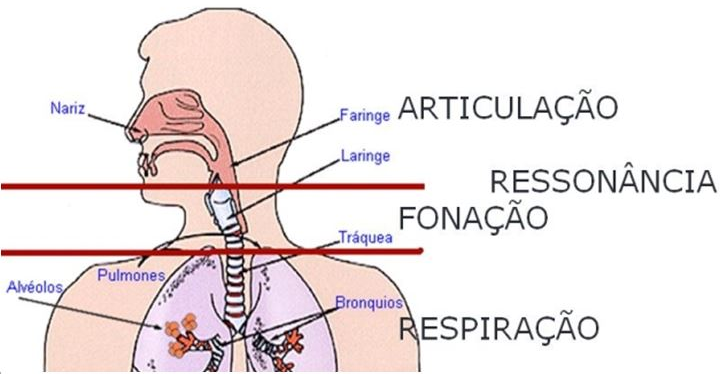
\includegraphics[width=13cm]{figuras/fisiologia-da-voz.png}		\caption{Fisiologia da voz (extra\'{i}do de  \cite{voz}).}
\label{figura:trato_vocal}
\end{figure}
%%%%%%%%%%%%%%%%%%%%%%%%%%%%%%%%%%%%%%%%%%%%%%%%%%%%%%%%
% SECAO
%%%%%%%%%%%%%%%%%%%%%%%%%%%%%%%%%%%%%%%%%%%%%%%%%%%%%%%%
\section{Sinais Digitais}
\label{sinais_digitais}
\par Os dados podem ser representados de duas maneiras: anal\'{o}gica ou digital. Aquela, em geral, caracteriza-se por uma onda eletromagn\'{e}tica que pode assumir infinitos valores ao longo do tempo, sendo a voz humana como \'{e} naturalmente encontrada na natureza, um exemplo. Esta, por outro lado, corresponde a um conjunto de valores com precis\~{a}o finita obtidos por um processo de amostragem temporal. Em outras palavras, o sinal digital que n\~{a}o seja oriundo de um processo de s\'{i}ntese, corresponde ao sinal anal\'{o}gico discretizado no tempo e quantizado em termos de amplitudes. 
\\
\par Particularmente, para se realizar uma an\'{a}lise em um sinal anal\'{o}gico em um computador, \'{e} necess\'{a}rio realizar a sua convers\~{a}o para a forma digital, uma vez que os computadores possuem uma capacidade finita de processamento, n\~{a}o sendo poss\'{i}vel assim processar os infinitos pontos de um sinal anal\'{o}gico. Tal processo de convers\~{a}o \'{e} denominado de digitaliza{\c c}\~{a}o, que \'{e} realizado em tr\^{e}s etapas. Na figura \ref{figura:quantizacao} s\~{a}o apresentados os processos de amostragem e de quantiza{\c c}\~{a}o, que ser\~{a}o comentados a seguir.
\begin{figure}[H]
\centering % para centralizarmos a figura
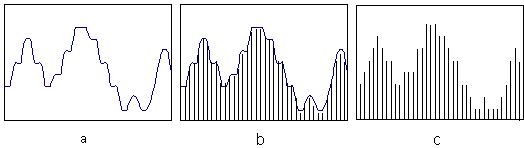
\includegraphics[width=13cm]{figuras/quant_amost.png} % leia abaixo
\caption{(a) Sinal na forma anal\'{o}gica. (b) Amostragem. (c) Quantiza{\c c}\~{a}o (extra\'{i}do de \cite{imagem_quantizacao}).}
\label{figura:quantizacao}
\end{figure}
\begin{enumerate}
\item{} \textbf{amostragem:} consiste no processo de obter amostras de um sinal anal\'{o}gico em instantes de tempo com espa{\c c}os iguais. Vale ressaltar que para se obter sucesso nesse processo de amostragem, \'{e} necess\'{a}rio seguir o Teorema de Nyquist \cite{deng}. Tal teorema define que, para realizar a amostragem de um sinal, \'{e} necess\'{a}rio no m\'{i}nimo ter uma taxa de amostras igual a duas vezes a m\'{a}xima frequ\^{e}ncia do sinal anal\'{o}gico. Caso n\~{a}o se obtenha tal taxa de amostragem ocorrer\'{a} um efeito chamado de \textit{aliasing}, que consiste na medi{\c c}\~{a}o erronea de uma frequ\^{e}ncia mais alta como sendo mais baixa. Um bom exemplo da aplica{\c c}\~{a}o de tal teorema \'{e} a digitaliza{\c c}\~{a}o da voz humana, que possui uma frequ\^{e}ncia m\'{a}xima em torno de 4 KHz. Logo, para realizar amostragem desses sinais, \'{e} necess\'{a}rio no m\'{i}nimo uma taxa de 8 mil amostras por segundo;
\item{} \textbf{quantiza{\c c}\~{a}o:} consiste na atribui{\c c}\~{a}o de valores discretos para as amplitudes do sinal anal\'{o}gico, que pertencem a um intervalo cont\'{i}nuo de valores. Cada amplitude \'{e} alocada ao n\'{i}vel de valor discreto mais pr\'{o}ximo, o que diminui assim os erros absolutos. Vale ressaltar que o n\'{u}mero de n\'{i}veis \'{e} definido pelo n\'{u}mero de \textit{bits} que ser\~{a}o utilizados na etapa posterior de codifica{\c c}\~{a}o, ou seja, ${2^n}$, sendo ${n}$ o n\'{u}mero de bits que ser\'{a} usado. De modo geral, nos sinais ac\'{u}sticos, \'{e} utilizada a quantiza{\c c}\~{a}o de 16 \textit{bits}. Em outras palavras, as amplitudes de cada amostra podem assumir ${2^{16}} = 65536$ valores distintos; 
\item{}	\textbf{codifica{\c c}\~{a}o:} etapa que consiste na modifica{\c c}\~{a}o de um sinal para uma aplica{\c c}\~{a}o espec\'{i}fica, como por exemplo o armazenamento ou transmiss\~{a}o de dados.
\end{enumerate}
\par Neste trabalho, todos os sinais de voz originalmente anal\'{o}gicos foram digitalizados para permitir manipula\c{c}\~{a}o por interm\'{e}dio computacional.  
%%%%%%%%%%%%%%%%%%%%%%%%%%%%%%%%%%%%%%%%%%%%%%%%%%%%%%%%
% SECAO
%%%%%%%%%%%%%%%%%%%%%%%%%%%%%%%%%%%%%%%%%%%%%%%%%%%%%%%%
\section{Arquivos Ac\'{u}sticos no Formato \textit{WAVE}}
\label{secao_formato wave}
\par\textit{Waveform audio file format}, abreviado de \textit{WAVE} ou simplesmente \textit{WAV}, \'{e} um tipo de formato de arquivos de \'{a}udio que foi desenvolvido pela \textit{Microsoft} em conjunto com a IBM. O formato \textit{WAVE} \'{e} amplamente utilizado em uma variedade de trabalhos, sejam eles cient\'{i}ficos ou profissionais, por permitir uma fiel representa\c{c}\~{a}o dos dados digitalizados, que n\~{a}o sofrem compress\~{a}o. \\
\par Na Tabela \ref{tabelawav}, a estrutura de um arquivo \textit{WAVE} est\'{a} descrita. Basicamente, o arquivo \'{e} dividido em dois grandes blocos, sendo o primeiro bloco um cabe{\c c}alho \textit{Rich Information File Format} (RIFF) e o segundo bloco, por sua vez dividido em dois sub-blocos, um conjunto de informa\c{c}\~{o}es referentes ao arquivo seguido dos dados brutos.
\\
\par Vale ressaltar que a quantiza\c{c}\~{a}o mais comum para cada amostra de um  arquivo \textit{WAVE} \'{e} normalmente de 8 \textit{bits} ou 16 \textit{bits}. No primeiro caso, existem 256 op\c{c}\~{o}es para cada amostra do sinal, sendo 127 positivos e 128 negativos. No segundo caso, por outro lado, s\~{a}o 65536 possibilidades, com 32767 positivos e 32768 negativos. Particularmente para a quantiza\c{c}\~{a}o de 16 \textit{bits}, \'{e} utilizada a codifica{\c c}\~{a}o de complemento de 2 para representar cada valor da amplitude do sinal. Assim, o valor do \textit{bit} mais significativo representa se o sinal \'{e} negaivo ou positivo. Neste trabalho foi utilizado o formato \textit{WAVE} de 16 \textit{bits} \textit{Pulse-code Modulation} (PCM), ou seja, sem compress\~{a}o. 
\begin{table}
	\centering
	\caption{Estrutura de um arquivo \textit{WAVE}}
	\begin{tabular}{|c|c|c|l|}
		\hline
		\hline
		\textbf{Classe} & \textbf{Posi\c{c}\~{a}o \textit{(bytes)}} & \textbf{Tamanho \textit{(bytes)}} & \textbf{Descri\c{c}\~{a}o}\\
		\hline
		\hline
		Cabe\c{c}alho & 0 & 4 & identificador do cabe\c{c}alho: ``RIFF''\\
		\hline
		Cabe\c{c}alho & 4 & 4 & Tamanho do arquivo \\
		\hline
		Cabe\c{c}alho & 8 & 4 & identificador ``\textit{WAVE}''\\
		\hline
		\hline
		Formato & 12 & 4 & identificador do segundo bloco: ``fmt''\\
		\hline
		Formato & 16 & 4 & tamanho do bloco sem o identificador\\
		\hline
		Formato & 20 & 2 & exist\^{e}ncia ou n\~{a}o de compress\~{a}o\\
		\hline
		Formato & 22 & 2 & quantidade de canais\\
		\hline
		Formato & 26 & 4 & taxa de amostragem\\
		\hline
		Formato & 30 & 4 & taxa de \textit{bytes}\\
		\hline
		Formato & 32 & 2 & quantidade de \textit{bytes} para uma amostra\\
		\hline
		Formato & 34 & 2 & quantidade de \textit{bits} para cada amostra\\
		\hline
		\hline
		Dados & 36 & 4 & identificador do terceiro bloco: ``\textit{data}''\\
		\hline
		Dados & 40 & 4 & tamanho do bloco sem o identificador\\
		\hline
		Dados & 44 & 4 & sinaliza o in\'{i}cio dos dados brutos \\
		\hline
	\end{tabular}
	\label{tabelawav}
\end{table}  
%%%%%%%%%%%%%%%%%%%%%%%%%%%%%%%%%%%%%%%%%%%%%%%%%%%%%%%%
% SECAO
%%%%%%%%%%%%%%%%%%%%%%%%%%%%%%%%%%%%%%%%%%%%%%%%%%%%%%%%
\section{Reconhecimento de Padr\~{o}es e Vetores de Caracter\'{i}sticas}
\label{reconhecimento_padroes_vetores_caracteristicas}
\par Na \'{a}rea de computa\c{c}\~{a}o, reconhecer um padr\~{a}o consiste, normalmente, em classificar sinais como pertencentes a determinadas classes ou categorias com base na extra{\c c}\~{a}o de caracter\'{i}sticas relevantes dos mesmos. De modo geral, o processo de classifica\c{c}\~{a}o consiste das seguintes fases: 
\begin{itemize}
\item{}\textbf{extra{\c c}\~{a}o das caracter\'{i}sticas:} principal etapa de todo o processo de reconhecimento de padr\~{o}es, consiste na redu{\c c}\~{a}o de dimensionalidade do sinal objetivando preservar elementos de fundamental interesse para a classifica\c{c}\~{a}o, compondo assim o vetor de caracter\'{i}sticas. Caso esse processo seja mal elaborado,  perder-se-\~{a}o caracter\'{i}sticas significativas, o que pode tornar a classifica{\c c}\~{a}o dispendiosa. Portanto, \'{e} necess\'{a}rio ter um conhecimento espec\'{i}fico sobre o problema, para poder realizar a redu{\c c}\~{a}o de dimensionalidade sem que ocorr\'{a} perdas de informa{\c c}\~{o}es relevantes, presando ainda pela redu\c{c}\~{a}o do esfor{\c c}o computacional;
\item{}\textbf{classifica{\c c}\~{a}o do sinal:} etapa que determina os procedimentos para realizar a classifica{\c c}\~{a}o do sinal em si, agora representado pelo seu vetor de caracter\'{i}sticas. De modo geral, os algoritmos de classifica\c{c}\~{a}o podem ser dos tipos \textit{pattern-matching} e \textit{knowledge-based}. No primeiro caso, as t\'{e}cnicas s\~{a}o mais elementares e n\~{a}o requerem treinamento pr\'{e}vio, isto \'{e}, nenhuma estat\'{i}stica sobre os dados a serem classificados \'{e} realizada. Por outro lado, no segundo caso, os algoritmos requerem um treinamento pr\'{e}vio levando em conta os padr\~{o}es a serem classificados, podendo ser:
		\begin{itemize}
		\item{}\textbf{treinamento supervisionado:} seu funcionamento \'{e} baseado em exemplos de entradas e sa\'{i}das previamente conhecidos, o que permite assim aprender uma regra gen\'{e}rica para classificar as entradas posteriores;
		\item \textbf{treinamento n\~{a}o supervisionado:} ao contr\'{a}rio da aprendizagem supervisionada, esta t\'{e}cnica n\~{a}o se baseia em r\'{o}tulos previamente conhecidos para classificar os sinais.
		\end{itemize}
\end{itemize}
\par Neste trabalho, o algoritmo particular a ser utilizado como classificador ser\'{a} determinado mediante a an\'{a}lise gr\'{a}fica dos vetores de caracter\'{i}sticas. Vetores com padr\~{o}es claramente distingu\'{i}veis podem fazer uso de t\'{e}cnicas mais modestas, isto \'{e}, \textit{pattern-matching} tal como a Dist\^{a}ncia Euclidiana. Por outro lado, vetores com padr\~{o}es similares entre as classes requerem classificadores mais elaborados, isto \'{e}, do tipo \textit{knowledge-based}, tal como uma rede neural artificial. 
%%%%%%%%%%%%%%%%%%%%%%%%%%%%%%%%%%%%%%%%%%%%%%%%%%%%%%%%
% SECAO
%%%%%%%%%%%%%%%%%%%%%%%%%%%%%%%%%%%%%%%%%%%%%%%%%%%%%%%%
\section{O Conceito de Energia}
\par A defini{\c c}\~{a}o de energia est\'{a} relacionada ao conceito de potencial para realizar trabalho. Neste projeto, a energia ser\'{a} considerada como a capacidade das estruturas voc\'{a}licas e dos pulm\~{o}es de produzir um sinal ac\'{u}stico. Na equa{\c c}\~{a}o \ref{eqenergia}, define-se a energia total $E(s[\cdot])$ de um dado sinal ac\'{u}stico digitalizado $s[\cdot]$ de tamanho $M$.
\begin{equation}
E(s[\cdot])=\sum_{i=0}^{M-1} (s_i)^2
\label{eqenergia}
\end{equation}
\par Para realizar a captura das caracter\'{i}ticas dos sinais, foi utilizado o m\'{e}todo $A_3$ definido em \cite{tut_energia}. Tal m\'{e}todo baseia-se em determinar comprimentos proporcionais para atingir n\'{i}veis predefinidos da energia do sinal que se encontra em an\'{a}lise. $A_3$ \'{e} ideal para avaliar os n\'{i}veis de energia de um sinal de voz digitalizado que foi gerado por um agente.
\\
\par Vale ressaltar que $A_3$ requer a defini\c{c}\~{a}o de um n\'{i}vel cr\'{i}tico de energia, $C$, que varia de 0 a 100\%. $A_3$ extrai um vetor de caracter\'{i}sticas dividindo o sinal original em partes proporcionais ao valor de $C$, ou seja, $K \cdot C$, sendo $K=1, 2, ...$ e ($K \cdot C < 100\%$). Assim, por exemplo, se $C=5\%$ e o vetor de caracter\'{i}sticas for designado por $f[\cdot]$, tem-se:
\begin{itemize}
\item{}$f_0$ corresponde a fra\c{c}\~{a}o do comprimento total do sinal original, a partir do in\'{i}cio, necess\'{a}ria para alcan\c{c}ar $1 \cdot 5 = 5\%$ da energia total do sinal; 
\item{}$f_1$ corresponde a fra\c{c}\~{a}o do comprimento total do sinal original, a partir do in\'{i}cio, necess\'{a}ria para alcan\c{c}ar $2 \cdot 5 = 10\%$ da energia total do sinal; 
\item{}$f_2$ corresponde a fra\c{c}\~{a}o do comprimento total do sinal original, a partir do in\'{i}cio, necess\'{a}ria para alcan\c{c}ar $3 \cdot 5 = 15\%$ da energia total do sinal; 
\item{}...
\item{}$f_{18}$ corresponde a fra\c{c}\~{a}o do comprimento total do sinal original, a partir do in\'{i}cio, necess\'{a}ria para alcan\c{c}ar $19 \cdot 5 = 95\%$ da energia total do sinal. 
\end{itemize}

\par Na figura \ref{figura:A3}, pode-se observar uma ilustra{\c c}\~{a}o do funcionamento de $A_3$.

\begin{figure}[H]
	\centering
	\includegraphics[width=18cm]{figuras/A3_energia.png}
	\caption{$A_3$ (extra\'{i}do de \cite{tut_energia})}
	\label{figura:A3}
\end{figure}

%%%%%%%%%%%%%%%%%%%%%%%%%%%%%%%%%%%%%%%%%%%%%%%%%%%%%%%%
% SECAO
%%%%%%%%%%%%%%%%%%%%%%%%%%%%%%%%%%%%%%%%%%%%%%%%%%%%%%%%
\section{O Conceito de \textit{Zero-crossing Rate} (ZCR)}

\par A Taxa de Cruzamento por Zeros ou \textit{Zero-Crossing Rate} - ZCR - \'{e} utilizada para definir quantas vezes a onda de um sinal cruza a amplitude zero. Pode-se tamb\'{e}m definir ZCR de acordo com a equa{\c c}\~{a}o \ref{eqzrc}, onde S[.] = $\{S_0, S_1, ..., S_{M-1}\}$ \'{e} um sinal discretizado de tamanho M$>$1 e sign(x) =
$
\begin{cases}
	\ \ 1, & se \ x \geqslant 0; \\
	-1, & caso \ contr\acute{a}rio.
\end{cases}
$

\par Para um sinal discreto, pode-se calcular o ZCR observando a mudan{\c c}a do sinal de negativo para positivo, ou vice-versa, considerando as amostras vizinhas.
\par De modo geral, os sons voc\'{a}licos est\~{a}o concentrados em baixas frequ\^{e}ncias, o que implica que se o ZCR for baixo pode-se classificar o som voc\'{a}lico, caso contr\'{a}rio como n\~{a}o voc\'{a}lico.

\begin{equation}
ZRC(S[.]) = \frac{1}{2} \sum_{j=0}^{M-2}|sign(S_j)-sign(S_{j+1})|
\label{eqzrc}
\end{equation}

\par Neste trabalho o conceito de ZCR foi utilizado com base no m\'{e}todo $B_3$ definido em \cite{tut_zcr}. Ele consiste em determinar comprimentos ou \'{a}reas proporcionais de um sinal que s\~{a}o requeridos para alcan{\c c}ar porcentagens pr\'{e}definidas do total de ZCR, o que torna este m\'{e}todo bem semelhante ao $A_3$ \cite{tut_energia}. $B_3$ \'{e} ideal para inspecionar a consist\^{e}ncia na frequ\^{e}ncia de uma entidade f\'{i}sica respons\'{a}vel por gerar S[.].
\par Assim como foi definido em $A_3$, $B_3$ requer que seja estabelecido um n\'{i}vel cr\'{i}tico de ZCR, C, que pode variar de 0 a $100\%$ e a partir disso, pode-se definir um vetor de caracter\'{i}sticas $f$[.] de tamanho T, conforme a seguir:

\begin{itemize}
	\item {} $f_0$ equivale a fra{\c c}\~{a}o de comprimento de S[.], a partir do seu in\'{i}cio at\'{e} alcan{\c c}ar C$\%$ do total de ZCR;	
	\item {} $f_1$ equivale a fra{\c c}\~{a}o de comprimento de S[.], a partir do seu in\'{i}cio at\'{e} alcan{\c c}ar $2 \cdot C\%$ do total de ZCR;	
	\item {} ...	
	\item {} $f_T-1$ equivale a fra{\c c}\~{a}o de comprimento de S[.], a partir do seu in\'{i}cio at\'{e} alcan{\c c}ar $T \cdot C\%$ do total de ZCR, de modo que $T \cdot C  < 100 \%$;
\end{itemize}

\par Na figura \ref{figura:B3} pode-se observar uma ilustra{\c c}\~{a}o do funcionamento do m\'{e}todo $B_3$. Al\'{e}m disso, pode-se definir T do seguindo modo:
T =
$
\begin{cases}
\ \frac{100}{C} - 1, & se \ C \ \acute{e} \ m\acute{u}ltiplo \ de \ 100; \\
\floor{\frac{100}{C}}, & caso \ contr\acute{a}rio.
\end{cases}
$

\begin{figure}[H]
	\centering
	\includegraphics[width=18cm]{figuras/B3.png}
	\caption{$B_3$ (extra\'{i}do de \cite{tut_zcr})}
	\label{figura:B3}
\end{figure}




%%%%%%%%%%%%%%%%%%%%%%%%%%%%%%%%%%%%%%%%%%%%%%%%%%%%%%%%
% SECAO
%%%%%%%%%%%%%%%%%%%%%%%%%%%%%%%%%%%%%%%%%%%%%%%%%%%%%%%%
\section{Classifica\c{c}\~{a}o baseada em dist\^{a}ncias}
\label{similaridade_baseada_em_distancias}
\par Quando \'{e} necess\'{a}rio agrupar vetores de caracter\'{i}sticas, normalmente utiliza-se como quesito a similaridade ou dissimilaridade entre os mesmos. Em espec\'{i}fico, para avaliar similaridades, uma s\'{e}rie de m\'{e}todos podem ser utilizados. No escopo das t\'{e}cnicas \textit{pattern-matching}, a dist\^{a}ncia Euclidiana \'{e} uma das mais cl\'{a}ssicas possibilidades sendo amplamente utilizada na literatura, com \cite{Marcel_Kfouri} e \cite{Ana_Paula} sendo alguns dos in\'{u}meros exemplos de trabalhos que utilizam a referida t\'{e}cnica. De acordo com a equa{\c c}\~{a}o \ref{eqdist}, onde P = $\{P_1, P_2, ..., P_n\}$ e Q = $\{Q_1, Q_2, ..., Q_n\}$ s\~{a}o dois vetores de caracter\'{i}sticas que distam $d$ unidades um do outro. A similaridade entre dois objetos ser\'{a} m\'{a}xima quando $P = Q$, implicando que $d=0$.
\begin{equation}
d(P, Q) = \sqrt{(P_1-Q_1)^2 + (P_2-Q_2)^2 + ... + (P_n-Q_n)^2} =\sqrt{\sum_{i = 1}^{n}(P_i-Q_i)^2} \qquad.
\label{eqdist}
\end{equation}
\par Uma variante da dist\^{a}ncia Euclidiana \'{e} a dist\^{a}ncia absoluta. Tal t\'{e}cnica utiliza o m\'{o}dulo da diferen{\c c}a entre dois n\'{u}meros para realizar a medi{\c c}\~{a}o da similaridade, conforme \'{e} mostrado na equa{\c c}\~{a}o \ref{eqdistab}. Assim como no caso anterior, caso a diferen{\c c}a seja igual a zero, tem-se que os dois vetores comparados s\~{a}o id\^{e}nticos.
\begin{equation}
d = \sum_{i = 1}^{n} | P_i-Q_i | \qquad.
\label{eqdistab}
\end{equation}
%%%%%%%%%%%%%%%%%%%%%%%%%%%%%%%%%%%%%%%%%%%%%%%%%%%%%%%%
% SECAO
%%%%%%%%%%%%%%%%%%%%%%%%%%%%%%%%%%%%%%%%%%%%%%%%%%%%%%%%
\section{Classifica\c{c}\~{a}o baseada em redes neurais}
\par Uma Rede Neural Artificial (RNA) \'{e} composta por dois elementos principais que s\~{a}o intimamente relacionados: A arquitetura da rede e o algoritmo de aprendizado. Esse por sua vez, \'{e} tipicamente organizado em at\'{e} tr\^{e}s camadas, com unidades que podem estar ligadas \`{a}s unidades da camada posterior. Na figura \ref{figura:rede} \'{e} apresentada um exemplo de uma arquitetura de RNA. 


\begin{figure}[H]
	\centering
	\includegraphics[width=10cm]{figuras/rede_neural.png}
	\caption{Exemplo de uma arquitetura de uma RNA}
	\label{figura:rede}
\end{figure}

\par Normalmente, as camadas s\~{a}o classificadas como segue:
\begin{itemize}
	\item {} \textbf{Camada de entrada:} \'{E} nessa camada que os padr\~{o}es ser\~{a}o apresentadas \`{a} rede.
	\item {} \textbf{Camada Intermedi\'{a}ria:} \'{E} respons\'{a}vel por realizar a maior parte do processamento, atrav\'{e}s das conex\~{o}es ponderadas.
	\item {} \textbf{Camada de sa\'{i}da:} Tem como funcionalidade concluir e apresentar o resultado final obtido pelo processamento. 
\end{itemize}

\par Vale ressaltar que os n\'{o}s da estrutura representado em \ref{figura:rede} s\~{a}o considerados como neur\^{o}nios, e toda informa{\c c}\~{a}o que passa por uma conex\~{a}o localizada entre aqueles leva \`{a} gera{\c c}\~{a}o de sinapses. Al\'{e}m disso, as RNAs funcionam de modo distribu\'{i}do e paralelo, de tal forma que cada n\'{o} possui capacidade para realizar processamento.

\par Por fim, a outra entidade elementar de um RNA \'{e} o algoritmo de aprendizagem que, por sua vez, tem como objetivo adquirir conhecimento do ambiente. Em outras palavras, adapta os pesos das conex\~{o}es aos est\'{i}mulos ou entradas captadas pelo ambiente de modo iterativo.  Os algoritmos de aprendizagem podem ser classificados nos seguintes paradigmas: supervionado e n\~{a}o supervionado, conforme mencionado na se{\c c}\~{a}o \ref{reconhecimento_padroes_vetores_caracteristicas}.

\par Neste trabalho, conforme j\'{a} mencionado, dependendo da an\'{a}lise gr\'{a}fica dos vetores de caracter\'{i}sticas, poder\'{a} a vir ser utilizada uma m\'{a}quina de vetor suporte (SVM - \textit{Support Vector Machine}) ou uma RNA para realizar as classifica{\c c}\~{o}es e reconhecimento dos comandos.
\par A SVM tem como principal caracter\'{i}stica ser um classificador bin\'{ario} de modo que consegue realizar a distin{\c c}\~{a}o de duas classes por uma fun{\c c}\~{a}o induzida por meio de exemplos. Essa distin{\c c}\~{a}o \'{e} obtida pela procura de um hiperplano \'{o}timo, conforme pode ser observado na figura \ref{figura:hiperplano}, na qual c\'{i}rculos verdes e amarelos representam cada uma das classes e as linhas solidas representam as separa{\c c}\~{o}es entre os planos.

\begin{figure}[H]
	\centering
	\includegraphics[width=10cm]{figuras/SVM.png}
	\caption{Hiperplano \'{o}timo}
	\label{figura:hiperplano}
\end{figure}

\par Na figura \ref{figura:hiperplano}, pode-se analisar que existem v\'{a}rios classificadores lineares para separar as amostrar, mas h\'{a} somente um (linha vermelha) que maximiza a margem - dist\^{a}ncia m\'{a}xima entre um elemento mais pr\'{o}ximo de cada classe e o classificador. Esse por sua vez \'{e} comumente referenciado na literatura como hiperplano de separa{\c c}\~{a}o \'{o}timo, pois ele consegue, mesmo que intuitivamente, generalizar melhor que os demais classificadores. J\'{a} as linhas tracejadas passam por alguns pontos para ambas as classes, esses s\~{a}o chamados de vetores-suporte.


%%%%%%%%%%%%%%%%%%%%%%%%%%%%%%%%%%%%%%%%%%%%%%%%%%%%%%%%
% SECAO
%%%%%%%%%%%%%%%%%%%%%%%%%%%%%%%%%%%%%%%%%%%%%%%%%%%%%%%%
\section{Matrizes de Confus\~{a}o}
\par Uma matriz de confus\~{a}o \'{e} comumente utilizado para avaliar o desempenho obtido por um classificador \cite{Pattern_Recognition}, ao mostrar a quantidade de classifica{\c c}\~{o}es corretas versus as classifica{\c c}\~{o}es previstas para cada classe, sobre um determinado conjunto de exemplos.
\par Uma matriz de  confus\~{a}o M \'{e} uma matriz de duas dimens\~{o}es, com o mesmo n\'{u}mero de linhas e colunas (n x n), no qual cada linha i representa a classe real daquilo que est\'{a} sendo classificado, e cada coluna j representa classe identificada pelo classificador \cite{Joao_Vitor_Maschio}. A quantidade de acertos, para cada classe, se encontra na diagonal principal $m_{ij}$, com $i = j$. J\'{a} as demais c\'{e}lulas de M representam os erros de classifica{\c c}\~{a}o.

\begin{table}[H]
	\centering
	\caption{Exemplo de uma matriz de confus\~{a}o}
	\begin{tabular}{|c || c c c |}
		\hline
		& Bom dia, Logan & Vai chover? & Pesquisar\\
		\hline
		\hline
		Bom dia, Logan & 8 & 2 & 0\\
		\hline
		Vai chover? & 2 & 6 & 1 \\
		\hline
		Pesquisar & 0 & 0 & 10\\
		\hline
	\end{tabular}
	\label{matriz_confusao}
\end{table}


\par A tabela \ref{matriz_confusao} mostra um exemplo de uma poss\'{i}vel matriz de confus\~{a}o para o trabalho aqui proposto. Em \ref{matriz_confusao}, temos 3 comandos distintos a serem identificados pelo classificador. Pode-se observar que para o comando \textit{Bom dia, Logan}, obteve-se 8 acertos e 2 erros, no qual o classificador identificou o comando em quest\~{a}o como \textit{Vai chover?}. J\'{a} para o comando \textit{Pesquisar}, obteve-se 10 acertos e nenhum erro.

\par Portanto, pode-se concluir que o melhor caso de uma classifica{\c c}\~{a}o ocorre quando a diagonal principal de M \'{e} m\'{a}xima e as demais c\'{e}lulas da matriz est\~{a}o zeradas, em outras palavras, o classificador obteve $100\%$ de acur\'{a}cia.


%%%%%%%%%%%%%%%%%%%%%%%%%%%%%%%%%%%%%%%%%%%%%%%%%%%%%%%%
% SECAO
%%%%%%%%%%%%%%%%%%%%%%%%%%%%%%%%%%%%%%%%%%%%%%%%%%%%%%%%
\section{Trabalhos Correlatos}
\label{trabalhos_correlatos}
\par A \'{a}rea de ASR tem sido bastante estudada em diversas trabalhos. Nas monografias de conclus\~{a}o de curso referenciadas em \cite{Marcel_Kfouri,Vinicius_Francisco,Ana_Paula,Joao_Vitor_Maschio,Reconhecimento_Comandos_Falados_Portugues_Brasileiro,Reconhecimento_voz_palavras_isoladas,Reconhecimento_automatico_fala_computador,Reconhecimento_padrao_formato_wave} s\~{a}o estudados e implementadas t\'{e}cnicas para identifica\c{c}\~{a}o de palavras no \^{a}mbito de vocabul\'{a}rio restrito. Por outro lado, nos artigos \cite{reconhecimento_vocabulario_chines,Reconhecimento_vocabulario_russo}, os esfor{\c c}os s\~{a}o voltados para o reconhecimento de um amplo vocabul\'{a}rio, inclusive em idiomas distintos do Portugu\^{e}s.
\\
\par Particularmente em \cite{Marcel_Kfouri}, o autor utiliza conceitos como energia, limiar \textit{hard} e n\'{i}veis cr\'{i}ticos de energia, para elaborar um sistema  de reconhecimento de vocabul\'{a}rio restrito implementado na linguagem C/C++, com um classificador baseado em dist\^{a}ncia Euclidiana.
\\
\par Em \cite{Ana_Paula}, o autor utiliza duas abordagens diferentes para realizar o reconhecimento de voz, sendo a primeira baseada em algoritmos \textit{pattern-matching} e a outra em \textit{knowledge-based}. Ao final do trabalho, pode-se concluir e verificar que a segunda abordagem apresentou melhores resultados para uma base de algumas dezenas de palavras.
\\
\par No trabalho referenciado em \cite{Joao_Vitor_Maschio}, o autor prop\~{o}em um sistema para reconhecimento de voz independente do locutor. Para isso, o autor utiliza conceitos como ZCRs e energias para realizar o pr\'{e}-processamento, extra{\c c}\~{a}o de caracter\'{i}sticas e um classificador tamb\'{e}m baseado em dist\^{a}ncia Euclidiana, contando com acur\'{a}cias superiores a 90\% para uma base de dezenas de palavras.
\\
\par Na monografia documentada em \cite{Voice_recognition_Room_automation}, o autor desenvolve um sistema de reconhecimento de voz baseado em automa{\c c}\~{a}o residencial via \textit{wireless}. Para a elabora{\c c}\~{a}o desse projeto, o autor utiliza o dispositivo HM2007L IC, para assim realizar o reconheicmento de comandos simples, como ``acender'', ``apagar'', ``acender a luz'', entre outros, contando com o mesmo n\'{i}vel de acur\'{a}cia dos trabalhos anteriormente mencionados.
\\
\par Em \cite{Laughing_Voice_Recognition}, o objetivo do autor \'{e} melhorar a rela{\c c}\~{a}o homem-m\'{a}quina, e com isso, desenvolve-se um m\'{e}todo para reconhecimento de voz com o uso de caracter\'{i}sticas \textit{voice-likeness}. Alcan{\c c}a-se uma acur\'{a}cia superior a 90\% considerando centenas de termos. 
\\
\par No trabalho \cite{A_Smartphone-Based_Multi-Functional_Hearing}, o autor tem como objetivo desenvolver um sistema para \textit{smartphones}, multifuncional, que al\'{e}m de realizar o reconhecimento de voz, tamb\'{e}m fa{\c c}a a convers\~{a}o do di\'{a}logo reconhecido para texto.
\\
\par Em \cite{Reconhecimento_voz_palavras_isoladas}, o autor utiliza conceitos como \textit{Mel frequency cepstral coefficients} (MFCC) e  \textit{Hidden Markov Models} (HMMs) para reconhecer um restrito vocabul\'{a}rio que cont\'{e}m digitos de 0 a 9, alcan\c{c}ando acur\'{a}cia quase plena para algumas centenas de testes.
\\
\par No artigo cient\'{i}fico \cite{reconhecimento_vocabulario_chines}, \'{e} realizada uma compara{\c c}\~{a}o de desempenho de Modelos de Misturas Gaussianas com Redes Neurais Profundas para o reconhecimento de um amplo vocabul\'{a}rio Chin\^{e}s. Os autores demonstram que as redes profundas s\~{a}o superiores aos modelos Gaussianos na maior parte das situa\c{c}\~{o}es. 
\\
\par Em \cite{Reconhecimento_vocabulario_russo}, com o objetivo de melhorar a efic\'{a}cia do reconhecimento de um vocabul\'{a}rio Russo amplo, foram utilizadas t\'{e}cnicas \textit{knowledge-based} para modelagem de fonemas, alcan\c{c}ando-se uma acur\'{a}cia superior a 95\% para muitas centenas de testes.
\\
\par Finalmente, no trabalho a ser implementado nesta monografia, ser\'{a} adotada uma linha de racioc\'{i}nio similar aos trabalhos \cite{Marcel_Kfouri,Vinicius_Francisco,Ana_Paula}, onde os autores utilizam conceitos j\'{a} conhecidos e consolidados na literatura da \'{a}rea de reconhecimento de voz, tais como n\'{i}veis cr\'{i}ticos de energia, dist\^{a}ncia Euclidiana, entre outros. Particularmente, este trabalho diferencia-se daqueles por objetivar o reconhecimento de palavras, num vocabul\'{a}rio restrito, de modo \textbf{dependente}, e n\~{a}o independente, do locutor.
%%%%%%%%%%%%%%%%%%%%%%%%%%%%%%%%%%%%%%%%%%%%%%%%%%%%%%%%
% CAPITULO 3
%%%%%%%%%%%%%%%%%%%%%%%%%%%%%%%%%%%%%%%%%%%%%%%%%%%%%%%%
%%%%%%%%%%%%%%%%%%%%%%%%%%%%%%%%%%%%%%%%%%%%%%%%%%%%%%%%
\chapter{Detalhamento do Trabalho Proposto}
\label{cap3}
\thispagestyle{myheadings}
%%%%%%%%%%%%%%%%%%%%%%%%%%%%%%%%%%%%%%%%%%%%%%%%%%%%%%%%
% SECAO
%%%%%%%%%%%%%%%%%%%%%%%%%%%%%%%%%%%%%%%%%%%%%%%%%%%%%%%%
\section{Status do trabalho proposto e sua continuidade}
\par No momento no qual este cap\'{i}tulo foi escrito, a revis\~{a}o bibliogr\'{a}fica j\'{a} havia sido realizada, assim como a coleta e elabora{\c c}\~{a}o do banco de sinais de voz.
\\
\par Com rela\c{c}\~{a}o aos sinais, foram definidos os 11 comandos que ser\~{a}o reconhecidos pelo sistema, conforme j\'{a} mencionado. Os comandos foram gravados 10 vezes em diferentes dias e hor\'{a}rios, para obter se assim, uma melhor veracidade e fidelidade \`{a} voz do locutor, pois o mesmo pode sofrer altera{\c c}\~{o}es significativas com base na varia{\c c}\~{a}o do seu humor ou estado f\'{i}sico. A grava{\c c}\~{a}o dos sinais foi realizada em um ambiente fechado, para diminuir assim, a probabilidade de ru\'{i}dos. Todos os arquivos foram gravados no formato  \textit{WAVE} de 16 \textit{bits} PCM, com o aux\'{i}lio do editor de \'{a}udio \textit{Audacity}. Posteriormente, foi iniciada a extra{\c c}\~{a}o das caracter\'{i}sticas de todos os sinais.
\\
\par A continuidade do trabalho seguir\'{a} o seguinte cronograma proposto:

\begin{table}[H]
	\centering
	\caption{Cronograma para desenvolvimento do trabalho}
	\begin{tabular}{|c|c|c|c|c|c|}
		\hline
		Atividades & Julho & Agosto & Set & Out & 10 Nov \\
		\hline
		 Desenvolvimento & \cellcolor{blue!25} &\cellcolor{blue!25} & & &  \\
		\hline
		  Escrita do Cap\'{i}tulo 3 &  &  & \cellcolor{blue!25} &  &  \\
		  \hline
		  Escrita do Cap\'{i}tulo 4 & & & &\cellcolor{blue!25} & \\
		  \hline
		  Escrita do Cap\'{i}tulo 5 & & & & \cellcolor{blue!25} &\\
		  \hline
		  Corre{\c c}\~{o}es & & & & \cellcolor{blue!25} & \\
		  \hline
		  Entrega da Monografia & & & & & \cellcolor{blue!25} \\
		  \hline
	\end{tabular}
	\label{cronograma}
\end{table}

%%%%%%%%%%%%%%%%%%%%%%%%%%%%%%%%%%%%%%%%%%%%%%%%%%%%%%%%
%%%%%%%%%%%%%%%%%%%%%%%%%%%%%%%%%%%%%%%%%%%%%%%%%%%%%%%%
% REFERENCIAS
%%%%%%%%%%%%%%%%%%%%%%%%%%%%%%%%%%%%%%%%%%%%%%%%%%%%%%%%
%%%%%%%%%%%%%%%%%%%%%%%%%%%%%%%%%%%%%%%%%%%%%%%%%%%%%%%%
\renewcommand
\bibname{\centering{Refer\^{e}ncias}}
\addcontentsline{toc}{chapter}{Refer\^{e}ncias}
\begin{thebibliography}{00}
\thispagestyle{myheadings}
\bibliographystyle{abnt-num}

\bibitem{cpp} Dr. Gary J. Bronson. A First Book of C++, 2011. 4. ed. Course Technology.
\bibitem{deng} Dong Yu, Li Deng. Automatic Speech Recognition: A Deep Learning Approach. 1 ed. Springer, 2015.
\bibitem{iot}  Graham Meikle, Mercedes Bunz. The Internet of Things. 1 ed. Polity Press, 2017.

\bibitem{arquit}HARRIS, D.; HARRIS, S. \textbf{Digital Design and Computer Architecture}, 2.ed. Morgan Kaufmann, 2012. 

\bibitem{pattern_classification}DUDA, R.; HART, D.; STORK, D. \textbf{Pattern Classification}. 2 ed. New York: Wiley-Interscience, 2000.

\bibitem{Pattern_Recognition}THEODORIDIS, S.; KOUTROUMBAS, K. Pattern Recognition. 4. ed, Academic Press, 2008.

\bibitem{ieee} http://www.ieeexplore.ieee.org. Acesso em Abril de 2017.

\bibitem{sciencedirect} http://www.sciencedirect.com. Acesso em Abril de 2017.

\bibitem{webofscience} http://isiknowledge.com. Acesso em Abril de 2017.

\bibitem{bill}https://www.cnet.com/au/news/gates-still-finding-his-voice/. Entrevista com Bill Gates. Acesso em Abril de 2017.

\bibitem{tut_energia}GUIDO, R. C. A tutorial on signal energy and its applications. Neurocomputting, v. 179, p.264-282, 2016.
\bibitem{tut_zcr}GUIDO, R.C. ZCR-aided neurocomputing: a study with applications. \textit{Knowledge-based Systems}, v. 105, pp.248-269, 2016.


\bibitem{Marcel_Kfouri}DORDAN, M, K. Verifica{\c c}\~{a}o de Locutores dependente do discurso baseada na Evolu{\c c}\~{a}o do Esfor{\c c}o Voc\'{a}lico. IBILCE, UNESP, S\~{a}o Jos\'{e} do Rio Preto (Trabalho de Conclus\~{a}o de Gradua{\c c}\~{a}o em Ci\~{e}ncia da Computa{\c c}\~{a}o), 2015.


\bibitem{Vinicius_Francisco}SILVA, V. F. Identifica{\c c}\~{a}o e Classifica{\c c}\~{a}o de G\~{e}neros Musicais com Abordagens M\'{u}ltiplas de Reconhecimento de Padr\~{o}es. IBILCE, UNESP, S\~{a}o Jos\'{e} do Rio Preto (Trabalho de Conclus\~{a}o de Gradua{\c c}\~{a}o em Ci\~{e}ncia da Computa{\c c}\~{a}o), 2014.


\bibitem{Ana_Paula}CAOBIANCO, A. P. Compara{\c c}\~{a}o de Abordagens \textit{PatternMatching} e \textit{Knowledge-Based} para Reconhecimento de Locutor Dependente de Texto. IBILCE, UNESP, S\~{a}o Jos\'{e} do Rio Preto (Trabalho de Conclus\~{a}o de Gradua{\c c}\~{a}o em Ci\~{e}ncia da Computa{\c c}\~{a}o), 2011.


\bibitem{Joao_Vitor_Maschio}MASCHIO, J. V. D. Projeto e Implementa{\c c}\~{a}o Ac\'{u}stico-Computacional de Palavras Isoladas. IBILCE, UNESP, S\~{a}o Jos\'{e} do Rio Preto (Trabalho de Conclus\~{a}o de Gradua{\c c}\~{a}o em Ci\~{e}ncia da Computa{\c c}\~{a}o), 2017.


\bibitem{Reconhecimento_Comandos_Falados_Portugues_Brasileiro}LOUREIRO, W. d. F. Reconhecimento de Comandos Falados Portugu\^{e}s Brasileiro com Par\^{a}metros de Frequ\^{e}ncia e Tempo. IBILCE, UNESP, S\~{a}o Jos\'{e} do Rio Preto (Trabalho de Conclus\~{a}o de Gradua{\c c}\~{a}o em Ci\~{e}ncia da Computa{\c c}\~{a}o), 2015.


\bibitem{Voice_recognition_Room_automation}PAUL, A.; PANJA, M.; BAGCHI, M.; DAS, N.; MAZUMDER, R. M.; GHOSH, S. Voice Recognition Based Wireless Room Automation System. In: International Conference on Intelligent Control Power and Instrumentation, 2016.


\bibitem{Laughing_Voice_Recognition}SAKANO, T.; KIGAWA, T.; SUGIMOTO, M.; KUSUNOKI, F.; INAGAKI, F.; MIZOGUCHI, H. Laughing Voice Recognition Using Periodic Waveforms and Voice-likeness Features. \textit{In: Proceedings of the 2016 IEEE International Conference on Robotics and Biomimetics}. Qingdao, China, 2016.


\bibitem{A_Smartphone-Based_Multi-Functional_Hearing}CHERN, A.; TSAO, Y.; CHANG, R.; HSIU-WEN, C.; YING-HUI, L. A Smartphone-Based Multi-Functional Hearing Assistive System to Facilitate Speech Recognition in the Classroom. Dispon\'{i}vel em: $<$http://ieeexplore.ieee.org/document/7938619/$>$. Acesso em: 05 jun. 2017.


\bibitem{Reconhecimento_voz_palavras_isoladas}SILVA, A. G. d. Reconhecimento de Voz para Palavras Isoladas. Monografia (Gradua{\c c}\~{a}o em Engenharia da Computa{\c c}\~{a}o) - UFPE, Recife, 2009.


\bibitem{Reconhecimento_automatico_fala_computador}LOUZADA, J. Reconhecimento Autom\'{a}tico de Fala por Computador. Monografia(Gradua{\c c}\~{a}o em Ci\~{e}ncia da Computa{\c c}\~{a}o) - PUC, Goi\'{a}s, 2010.


\bibitem{Reconhecimento_padrao_formato_wave}Piccoli, E. E. M. Reconhecimento de Padr\~{a}o em \'{A}udio no Formato Wave. IBILCE, UNESP, S\~{a}o Jos\'{e} do Rio Preto (Trabalho de Conclus\~{a}o de Gradua{\c c}\~{a}o em Ci\~{e}ncia da Computa{\c c}\~{a}o), 2014.


\bibitem{reconhecimento_vocabulario_chines}LI, X.; YANG, Y.; PANG, Z.; WU, X. A Comparative Study on Selecting Acoustic Modeling Units in Deep Neural Networks Based large Vocabulary Chinese Speech Recognition. Neurocomputing, v. 170, p. 251-256, 2015.


\bibitem{Reconhecimento_vocabulario_russo}KARPOV, A.; MARKOV, K.; KIPYATKOVA, I.; VAZHENINA, D.; RONZHIN, A.; Large Vocabulary Russian Speech Recognition Using Syntactico-statistical language Modeling. Speech Communication, v.56, p.213-228, 2014.


\bibitem{imagem_quantizacao}$<$http://penta3.ufrgs.br/RNP/cap3/3.2\%20Audio/$>$. Acesso em: 20 Abril 2017.


\bibitem{voz}$<$http://www.koreapost.com.br/wp-content/uploads/2016/01/fisiologia-da-voz.jpg$>$. Acesso em: 18 Abril 2017. 

\end{thebibliography}
%%%%%%%%%%%%%%%%%%%%%%%%%%%%%%%%%%%%%%%%%%%%%%%%%%%%%%%%
%%%%%%%%%%%%%%%%%%%%%%%%%%%%%%%%%%%%%%%%%%%%%%%%%%%%%%%%
% APENDICE
%%%%%%%%%%%%%%%%%%%%%%%%%%%%%%%%%%%%%%%%%%%%%%%%%%%%%%%%
%%%%%%%%%%%%%%%%%%%%%%%%%%%%%%%%%%%%%%%%%%%%%%%%%%%%%%%%
\end{document}